\section{An overview of the Ground Handling tasks}
This section will describe which different tasks are done by the ground handling companies and how they are connected and dependent of each other.

In an interview made in Aalborg Airport with the COO, Kim Bergmann, it was found that many different airlines needs many different services and procedures done to an aircraft. There are though some most common and nearly only used tasks which will be covered in this section, but it is important to strech that any airline/ground handling company needs to be able to vairy and change these tasks since gound handling is a complex and large system. To give an overview of what tasks that are done to the aircrafts an overview of the aircraft has been made from the book Airport design and operation \cite{Airport design and operation} chapter 9 which decribes the ground handling process in detail. In graph \ref{B-777_Turnaround} we can see the different tasks done to an normal airplane during an end-station turnaround (a turnaround where passengers and luggage have arrived at their destination and new passengers, luggage and intentionally crew needs to board the flight).

\begin{figure}[H]
\centering
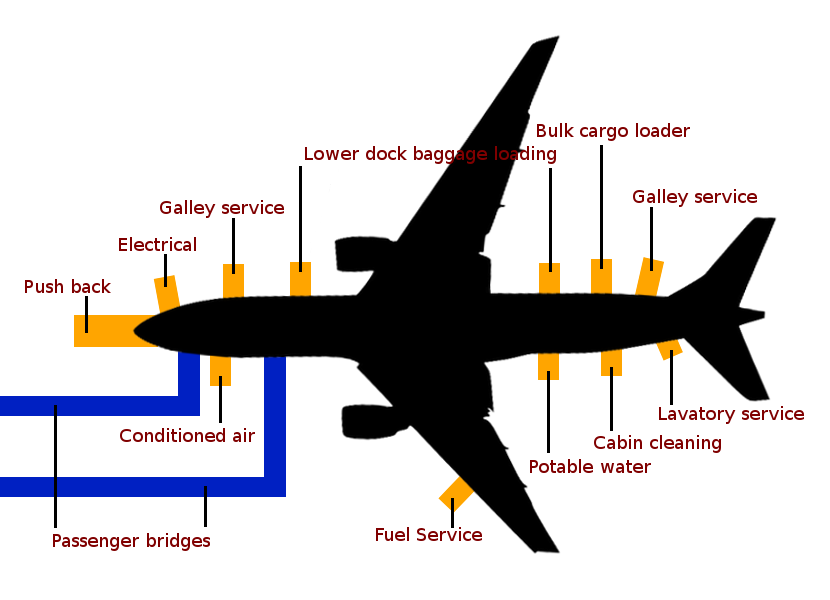
\includegraphics[width=\textwidth]{Grafik/B-777_Turnaround}
\caption{An overview of the different ground handling tasks done to an Boeing 777. http://pixabay.com/static/uploads/photo/2012/04/15/18/22/cloud-34787_640.png}
\label{B-777_Turnaround}
\end{figure}

The amount of tasks needing to be done to an airplane vary from company to company, airport to airport, time of day and ect., but this example is used to illustrate all of the categories. It is also shown where the different tasks are approximately placed on the Boeing-777, this position of cause vary from airplane to airplane and also the amount of cargo-storage areas inside the airplane and the need for either passenger bridges and/or stairs vary from airplane to airplane and also airport to airport. Also, the size of the different "vehicles" doing the tasks are not exact.

The next sections will now describe the different tasks, what they do and how they are done.

\subsection{Electricity}
This is ofteh the first point of ground handling, where the plane is connected to the airports powersupply. Here its batteries get charged and get ready for the next flight. The charging stations are almost exclusively stationary, and located at the front of the apron. This proccess can happen at the same time as all the following processes. 

\subsection{Galley service/catering}
The catering services are everything related to the food and drinks on the airplane. There is a lot of different ways to handle catering. SAS for example, provides free coffee on all of their flights, but most of their flights is only national, so there is no need for food. Other companies dealing with internation flights provide food for either all the passengers or to some, who pay in advance. This process can only happen after the passengers has left the plane.

\subsection{Conditioned air}


\subsection{Passenger bridges/stairs}
Passengers will leave different planes in different ways. They can leave through an aviobridge, they can leave by walking from the plane to terminal or on bigger airports they can be collected by a bus. This process typically happens before the fueling of the plane.

\subsection{Fuel service}
Fueling happens in different ways in different airports. In some airports pump vehechiels drive up to the planes and fuel them manually, while in other airports, stationary pumps are located on the individual aprons.

\subsection{Push back}
When all other procceses has been completed the airplane can take off. For this to happen a push back has to happen. This happens with the help of a specialced machine called a tractor. With the help of this machine the airplane is pushed to a point where it can easily taxi to the runway.



\subsection{Baggage and cargo loading and unloading}
\subsection{Potable water}
\subsection{Cabin cleaning}
\subsection{Lavatory service}
\subsection{Deicing}

\section{Relationship}
Many tasks needs to done before others can start, for instance you need to unload the current luggage/cargo before new can be loaded or as described in fuel service passengers normally needs to leave the airplane before the fueling process can be started. To give a clear and structured overview the total ground handling service is divided into 3 individual tracks.
